\section{Discussion}
\label{sec:discussion}

\subsection{Perfect coordination}
\label{sec:perfect-coordination}
We analyse the policy that agents learn with the VDN baseline and show their ability to achieve perfect coordination. VDN has been chosen over QMIX for interpretability reasons and because it has been the most successful algorithm in our tests. 

\paragraph{Level 6} Analysing the policy of the four agents after training for 1m steps, we can see that the agents understand the laser dynamics: they learn low $Q_i$-values for walking into deadly lasers and for releasing a laser beam on another agent (killing it). Agents red and yellow also learn to cooperate and block lasers for each other in order to reach the bottom half of the map, collect the gems and reach the exit tiles. We argue that agents learn perfect coordination and illustrate that behaviour in a simpler toy example illustrated in \autoref{fig:toy-example}, where agents must also block a laser.

\begin{figure}[t]
    \centering
    \begin{subfigure}[b]{0.24\textwidth}
         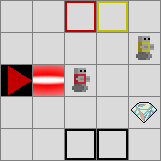
\includegraphics[width=\linewidth]{images/step_2.png}
         \caption{}
         \label{fig:step2-blocking}
    \end{subfigure}
    \begin{subfigure}[b]{0.24\textwidth}
         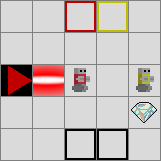
\includegraphics[width=\linewidth]{images/step_3.png}
         \caption{}
         \label{fig:step3-crossing}
    \end{subfigure}
    \begin{subfigure}[b]{0.24\textwidth}
         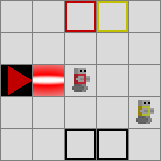
\includegraphics[width=\linewidth]{images/step_4.png}
         \caption{}
         \label{fig:step4-passed}
    \end{subfigure}
    \caption{Four consecutive states of an episode. Agent red blocks the laser for agent yellow and waits for the latter to have left the range of the blocked beam.}
    \label{fig:toy-example}
\end{figure}

\subsubsection{Toy example} Consider the toy example depicted in \autoref{fig:toy-example} with one laser and two agents. We train the agents for 160k steps and then analyse the $Q_i$-values during the steps concerned by perfect coordination in \autoref{tab:steps-qvalues}.


\begin{table}
    \centering
    \caption{$Q_i$-values from the successive states depicted in \autoref{fig:toy-example}. The highest $Q_i$-values are in bold.}
    \label{tab:steps-qvalues}
    \begin{tabular}{c|l|rrrrr}
         \textbf{State} & \textbf{Agent} & \textbf{North} & \textbf{South} & \textbf{West} & \textbf{East} & \textbf{Stay}\\
         \hline
         \multirow{2}{*}{\ref{fig:step2-blocking}}
         & \cellcolor{red!70} Red & -1.29 & -0.97 & 2.52 & 2.53 & \textbf{2.56} \\
         & \cellcolor{yellow!70} Yellow & 0.78 & \textbf{0.94} & 0.67 & 0.91 & 0.85\\
         \hline
         \multirow{2}{*}{\ref{fig:step3-crossing}}
         & \cellcolor{red!70} Red & 1.44 & 1.51 & 1.48 & 1.51 & \textbf{1.56} \\
         & \cellcolor{yellow!70} Yellow & 1.77 & \textbf{2.13} & 1.18 & 1.41 & 1.45\\
         \hline
         \multirow{2}{*}{\ref{fig:step4-passed}}
         & \cellcolor{red!70} Red & 1.15 & \textbf{1.36} & 1.16 & 1.19 & 1.25 \\
         & \cellcolor{yellow!70} Yellow & 0.71 & 1.42 & \textbf{1.49} & 1.42 & 1.41\\
    \end{tabular}
\end{table}

Starting with step \ref{fig:step2-blocking}, the red agent understands that releasing the laser beam has a much lower value than the other actions because it would likely kill agent yellow. The $Q_i$-values suggest that the \textit{credit} for killing an agent (and hence losing the game) is assigned to the one releasing the beam, not to the one walking in the laser span.
At step \ref{fig:step3-crossing}, the $Q_{i}$-values of agent yellow show that the yellow agent has a clear preference for the south action to collect one gem and close the gap with the exit. Meanwhile, agent red keeps blocking the laser as long as agent yellow stands in the range of the laser beam. With such behaviour similar to the one of level 6 for agent red and yellow, we conclude that agents achieve perfect coordination successfully.

\subsection{Interdependence}
\label{sec:discussion-interdependence}
As discussed in \autoref{sec:prop-interdependence}, agents interdependence introduces bottlenecks in the state space, making that category of environment challenging exploration tasks. We hypothesise that this difficulty of randomly stumbling on good policies contributes to the failure of PER: if agents never come across good policies, PER can never prioritise it. Across the 20 seeded runs with PER on level 6, we checked that at no single point in time, any episode ever reached an exit rate above 0.5. With RND however, agents \emph{very} occasionally reached an exit rate of 0.75, suggesting that RND might be pushed further.


\subsection{Zero-incentive dynamics}
\label{sec:discussion-zid}
We argue that the zero-incentive dynamics of LLE have a detrimental effect on $n$-step return and on PER because they accentuate the punishment of dying from lasers each in their own way.

With regard to PER, since walking into a laser either yields no reward or a punishment (as the definition of zero-incentive dynamics implies), PER is likely to give a higher priority to transitions where punishment has occurred rather than to transitions with a null reward. As a result, we hypothesise that in the early stages of the game, PER emphasises the fact that lasers can be deadly which results in agents being more reluctant to walk into lasers overall.

Looking into the poor performance of $n$-step return, we observe that agents are very likely to die by walking into a laser in their exploration phase. It is also very likely that this punishment is the only non-null reward signal within the $n$ last steps because of the reward sparsity and the zero-incentive dynamics of the environment.  Consequently, when this ``bad'' experience (caused by a poor policy or by random exploration) is then sampled from the replay buffer, the agents learn that the $n$ last actions eventually lead to punishment and their policy is therefore updated to be ``safer''. Our experimental results in Appendix~\ref{apx:n-step} support this explanation, as the mean score decreases when $n$ increases.

